\newcommand{\asampling}{\proc{Amostragens Adaptativas}}
\newcommand{\AS}{\proc{AdaptiveSampling}}

\chapter{Contagens por amostragens}

Este capítulo aborda uma outra solução para o problema da contagem distinta aproximada. O 
Capítulo~\ref{lab:flajolet-martin} apresentou o algoritmo da $\pcounting$, que estima o número de elementos distintos em 
um fluxo de dados com desvio padrão em torno de $0.78 / \sqrt{m}$. 

O algoritmo das $\asampling$ tem um desvio padrão de aproximadamente $1.20 / \sqrt{m}$~\citep{adptive:sampling:90}. 
As razões para estudarmos esse algoritmo mesmo que ele apresente um erro maior ficarão claras nas próximas seções.

\section{Algoritmo das $\asampling$}
\label{lab:chapter:04:01}

O algoritmo das $\asampling$ também se baseia em \hyperref[sec:flajolet-martin:pattern]{padrões de bits} dos hashes dos 
elementos examinados. Podemos dessa forma, considerar que os elementos que estamos contando são palavras binárias de 
tamanho infinito. 

Enquanto que no algoritmo da $\pcounting$, estávamos interessados na \textbf{aparição} de um elemento com 
prefixo da forma $0^*1$, no algoritmo das $\asampling$, queremos saber a \textbf{quantidade} de elementos com um certo 
prefixo $0^*$.

Nesse sentido, vamos manter um contador $\delta$ cujo valor inicialmente é zero, e uma lista que armazena elementos com 
prefixo $0^{\delta}$. Para cada elemento examinado, inserimos ele na lista se o prefixo dele for da forma $0^{\delta}$.
Quando essa lista tiver mais que $m$ elementos, incrementamos $\delta$ em 1 e passamos a manter 
somente elementos com prefixo $0^{\delta + 1}$.

Agora, suponha que em um dado momento do algoritmo, a lista tenha tamanho $l$ e estamos mantendo somente elementos com 
prefixos $0^{\delta}$. A probabilidade de um elemento ter um prefixo dessa forma é $1 / 2^{\delta}$, e consequentemente,
esperamos que a cada $2^{\delta}$ itens, pelo menos um item tenha um prefixo desse formato. Assim, se nossa lista tem
$l$ elementos com prefixo $0^{\delta}$, então devemos ter examinado pelo menos $2^{\delta} l$ itens, e este valor é 
justamente a estimativa para a quantidade de valores distintos.

O algoritmo $\AS$ recebe um fluxo $\Mbb$ com $n$ elementos distintos e um parâmetro $m$, que está relacionado com o 
consumo de memória do algoritmo e sua precisão. O algoritmo usa uma função de hash $h$ para associar de forma uniforme 
os elementos de~$\Mbb$ a inteiros de~$L$ bits, e quanto maior for este valor, menor será a quantidade de colisões. Por 
fim, o valor devolvido é um estimador~$\hat{n}$ para $n$ da forma $2^{\delta} l$, em que $l$ e $\delta$ indicam que 
estão sendo armazenados $l$ elementos cujos prefixos tem formato~$0^{\delta}$. 

\begin{codebox}
  \Procname{$\AS(\Mbb, m)$}
  \li $LIST \gets \emptyset$
  \li $\delta \gets 0$
  \li \For cada $x$ em $\Mbb$ 
  \li    \Do 
         \If $0^{\delta}$ é prefixo de $h(x)$ \textbf{e} $h(x) \not\in LIST$
  \li             \Then $LIST \gets LIST \cup \{ h(x) \}$
         \End
  \li    \While $|LIST| > m$                                   \label{li:as:while}
  \li    \Do
         $\delta \gets \delta + 1$
  \li    $TEMPLIST \gets \emptyset$
  \li    \For cada $y$ em $LIST$
  \li    \Do
            \If $0^{\delta}$ é prefixo de $h(y)$
  \li       \Then $TEMPLIST \gets TEMPLIST \cup \{ h(y) \}$
            \End
         \End
  \li    $LIST \gets TEMPLIST$
         \End 
      \End
  \li
  \Return $2^{\delta} |LIST|$   
  \End
\end{codebox}


\section{Vantagens das $\asampling$}
\label{lab:chapter:04:02}

Vamos simular um exemplo pequeno para ver o funcionamento do algortimo $\AS$. Assim, queremos estimar quantos elementos 
distintos o fluxo $\Mbb = \{ 36, 108, 41, 82, 71, 61, 5, 54, 10 \}$ possui. Vamos considerar que a função de hash~$h$ é
a identidade, ou seja, $h(x) = x$ para todo $x$ em $\Mbb$, e que $m = 3$. 

Inicialmente, a lista $LIST$ está vazia e $\delta = 0$. Na primeira iteração do algoritmo, temos que verificar se o 
prefixo da representação binária do elemento $36 = 001001_2$ é da forma $0^0$. Note que qualquer elemento passará nessa 
validação quando $\delta$ for zero, uma vez que, uma palavra binária precisar ter o prefixo $0^0$ significa que ela tem 
que começar com 0 zeros, ou seja, pode começar com 0 ou com 1. Dessa forma, podemos inserir o elemento $36$ na lista, de 
modo que $LIST = \{ 36 \}$. Na próxima iteração, temos que fazer a mesma verificação anterior, só que usando o item de 
valor 108. Novamente, como $\delta = 0$, podemos adicionar $108$ à lista. Analogamente, podemos incluir os elementos 
$41$ e $82$ em $LIST$. 

Contudo, na quarta iteração, entramos no \texttt{while} da linha~\ref{li:as:while}, já que $|LIST| = 4 > m = 3$. Por 
conta disso, incrementamos o valor de $\delta$ e devemos manter em $LIST$ somente aqueles valores cujos prefixos de suas 
representações binárias são da forma $0^{1}$. Vamos ver quais elementos estão em $LIST$:
\[ 
       LIST = \{ 36 = 001001_2, 108 = 0011011_2, 41 = 100101_2, 82 = 0100101_2 \} \  .        
\] 
Precisamos manter nessa lista, somente aqueles números com prefixos que começam com~0. Assim, temos que remover o valor 
41 de $LIST$. 

Continuando o exemplo, precisamos verificar se adicionaremos $71 = 1110001_2$ na lista. Agora, os elementos em $LIST$ 
precisam começar com zero, logo 71 não é inserido. A mesma situação ocorre para os valores $61 = 101111_2$ e 
$5 = 101_2$. Em seguida, podemos inserir $54 = 011011_2$ em $LIST$ e como novamente, $|LIST| = 4 > 3$, teremos que 
incrementar $\delta$ e filtrar os itens da lista. A lista atual é 
\[ \{ 36 = 001001_2, 108 = 0011011_2, 82 = 0100101_2, 54 = 011011_2 \} \ . \] 
Manteremos somentes os valores cujos prefixos binários se iniciam com dois zeros e portanto, 
\[ LIST = \{ 36 = 001001_2, 108 = 011011_2 \} \ . \]
Por fim, o valor $10 = 0101_2$ não é inserido na lista. E a estimativa para a quantidade de elementos distintos em 
$\Mbb$ é $2^{\delta} \times |LIST| = 2^2 \times 2 = 8$. Essa estimativa está cometendo um erro de um item, já que $\Mbb$
tem 9 itens distintos. 

O fato curioso desse exemplo acontece nas primeiras iterações, quando $\delta$ tem valor zero. Vimos que qualquer 
elemento de $\Mbb$ nessas primeiras iterações é inserido em $LIST$. Nessas situações, a estimativa do algoritmo é 
$2^{\delta} \times |LIST| = 2^{0} \times |LIST| = |LIST|$. Ou seja, para os primeiros $m$ itens distintos de $\Mbb$, a 
estimativa tem precisão de $100\%$. Isto é o principal diferencial do algoritmo das $\asampling$ para o algoritmo da 
$\pcounting$, que como foi visto em \hyperref[sec:fm:low_estimates]{Estimando valores pequenos com a $\pcounting$}, 
apresenta um erro muito grande quando queremos estimar cardinalidades baixas.

Outro fator importante de se destacar é que o estimador devolvido por $\AS$ é 
\textbf{não-viesado}~\citep{adptive:sampling:90}. Essa característica está relacionada com o fato do algoritmo das 
$\asampling$ poder estimar valores pequenos sem problemas.

\newpage
\section{Um, dois, três, \dots, repetido, \dots}

Nesta seção apresentaremos a implementação do algoritmo das \proc{Amostragens} \proc{Adaptativas} e experimentos.

\begin{lstlisting}[style=mypython,caption=Implementação do algoritmo $\AS$,captionpos=b, label=as:code]
class AdaptiveSampling:
    def __init__(self, m=64, L=64):
        self.delta: int = 0
        self.m: int = m
        self.L: int = L
        self.LIST: Set[int] = set()
   
    def zeros_no_prefixo(self, x: int):
        return (x & -x).bit_length() - 1

    def adiciona(self, x: int):
        if x not in self.LIST and self.zeros_no_prefixo(x) >= self.delta:
            self.LIST.add(x)

        while len(self.LIST) > self.m:
            self.delta = self.delta + 1
            temp: Set[int] = set()

            for y in self.LIST:
                if self.zeros_no_prefixo(y) >= self.delta:
                    temp.add(y)

            self.LIST = temp

    def conta(self):
        return (1 << self.delta) * len(self.LIST)
\end{lstlisting}

Vamos comentar alguns aspectos do código do Programa~\ref{as:code} baseado no algoritmo~$\AS$. O primeiro detalhe de 
implementação desse programa é que a função de hash~$h$ é implicitamente a função identidade, uma vez que, estamos 
supondo que os elementos inseridos são inteiros gerados uniformemente. O próximo detalhe é a estrutura de dados 
utilizada para representar a lista $LIST$. Foi escolhido um \proc{Set} para representá-la, que é uma estrutura padrão do 
\proc{Python} que permite inserir elementos e verificar se um elemento está presente nela em tempo constante. Dessa 
forma, a complexidade do método~\texttt{adiciona} é $O(1)$ amortizado.

Por fim, falta esclarecer como foi codificada a verificação se um inteiro tem prefixo da forma $0^{\delta}$, ou em 
outras palavras, se a representação binária de um inteiro começa com pelo menos $\delta$ zeros. Lembremos dessa forma, 
da função $\rho$ definida na Seção~\ref{sec:flajolet-martin:algorithm}. Essa função recebe um inteiro $x$ e devolve a 
posição indexada a partir do zero do bit menos significativo de $x$. Assim, $\rho(12) = \rho(0011_2) = 2$ e 
$\rho(24) = \rho(00011_2) = 3$. Note que a saída da função $\rho$ corresponde também a quantidade de bits zeros no 
prefixo da representação binário de um inteiro. Podemos, portanto, aproveitar o método $p$ da classe 
\texttt{ProbabilisticCounting} para implementar o método \texttt{zeros\_no\_prefixo} e agora, para verificar se um 
inteiro~$x$ tem prefixo da forma $0^{\texttt{delta}}$, basta testar se \texttt{zeros\_no\_prefixo(x)} é maior ou igual a
\texttt{delta}.

A partir deste ponto, apresentaremos experimentos do algoritmo das \proc{Amostragens} \proc{Adaptativas}, que serão os 
mesmos realizados na Seção~\ref{sec:fm:experiments}, só que utilizando a estrutura apresentada nesse capítulo. Assim, o 
primeiro experimento que veremos é observar a evolução das estimativas devolvidas pela estrutura
~\texttt{AdaptiveSampling} conforme mais itens são inseridos nela. Portanto, nas simulações realizadas, inserirmos um 
milhão de inteiros de 64 bits distintos gerados uniformemente em estruturas com $m = 64$ e $m = 1024$. E o mesmo gerador 
de números pseudo-aleatórios dos experimentos do algoritmo da~$\pcounting$ foi utilizado, ou seja, os mesmos elementos 
foram aproveitados.

Os resultados do primeiro experimento podem ser observados na Figura~\ref{fig:as:experimento:01}. É possível perceber
que a estrutura com o parâmetro $m$ maior teve uma precisão melhor que a estrutura com $m$ menor ao longo de toda a 
simulação. 

\begin{figure}
  \centering
  \begin{subfigure}{.5\textwidth}
    \centering
    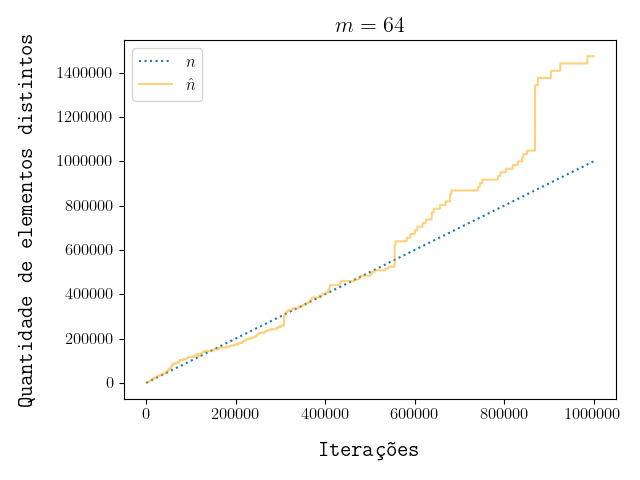
\includegraphics[width=\linewidth, height=4cm]{figuras/adaptive_sampling_full_64.png}
  \end{subfigure}%
  \begin{subfigure}{.5\textwidth}
    \centering
    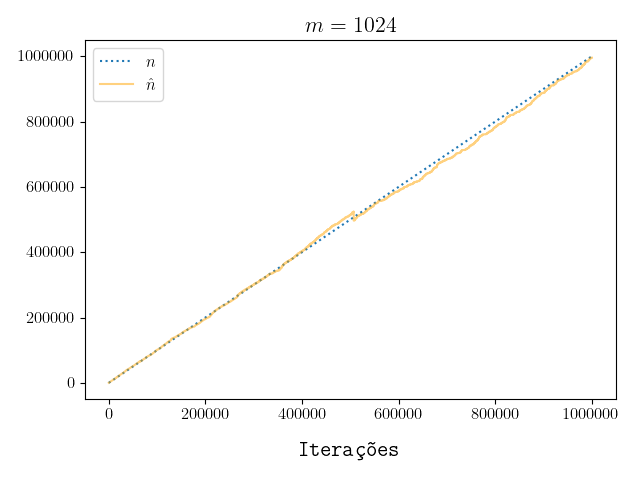
\includegraphics[width=\linewidth, height=4cm]{figuras/adaptive_sampling_full_1024.png}
  \end{subfigure}
  \caption{Primeiro experimento do algoritmo $\AS$. Foram inseridos em estruturas \texttt{AdaptiveSampling} com $m = 64$ 
  e $m = 1024$, um milhão de inteiros de 64 bits gerados uniformemente.}
  \label{fig:as:experimento:01}
\end{figure}


Os gráficos com a evolução do erro relativo do experimento anterior estão na Figura~\ref{fig:as:experimento:01:erro}.
O desvio padrão do algoritmo das $\asampling$ é $1.20/\sqrt{m}$. Portanto, para a estrutura com $m = 64$, o desvio 
padrão é de $15\%$. As estimativas devolvidas por essa estrutura ficaram entre dois desvios padrões na maior parte da 
simulação, apresentando um erro maior quando esta se aproximava do fim. Já a estrutura com $m = 1024$ tem desvio padrão 
de $3{,}75\%$, e a simulação dela teve valores que ficaram dentro de um desvio na maior parte das iterações.

\begin{figure}
  \centering
  \begin{subfigure}{.5\textwidth}
    \centering
    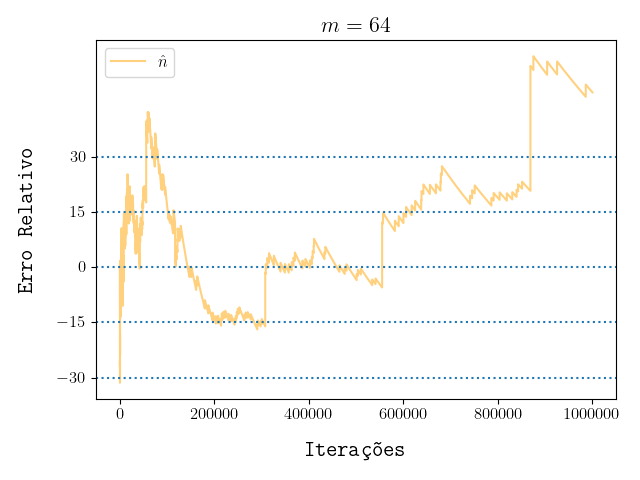
\includegraphics[width=\linewidth, height=4cm]{figuras/adaptive_sampling_erro_full_64.png}
  \end{subfigure}%
  \begin{subfigure}{.5\textwidth}
    \centering
    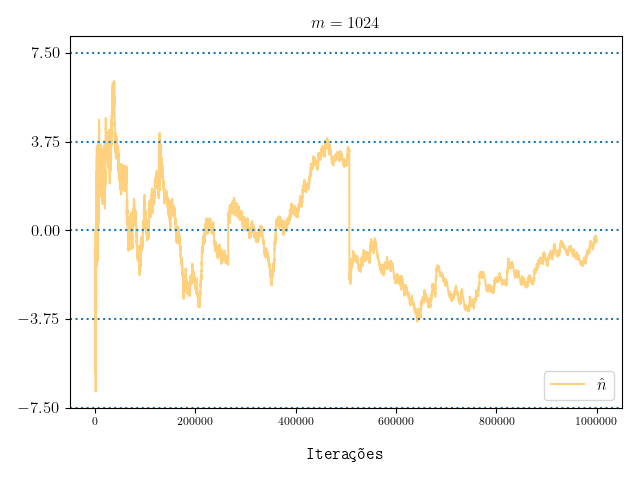
\includegraphics[width=\linewidth, height=4cm]{figuras/adaptive_sampling_erro_full_1024.png}
  \end{subfigure}
  \caption{Erro relativo do primeiro experimento do algoritmo $\AS$. Para $m = 64$, o erro ficou dentro de dois desvios
  padrões. Para $m = 1024$, a faixa de erro foi de um desvio padrão.}
  \label{fig:as:experimento:01:erro}
\end{figure}

Antes de passarmos para o segundo experimento, é interessante verificarmos se o que foi discutido na 
Seção~\ref{lab:chapter:04:02} pode ser observado nas simulações anteriores. Queremos, assim, averiguar se o algoritmo 
das~$\asampling$ funciona de fato para baixas cardinalidades. A Figura~\ref{fig:as:experimento:01:erro:first} tem
gráficos que destacam o erro relativo nas primeiras~256 iterações no caso da estrutura com $m = 64$ e nas primeiras~1024
iterações no caso da estrutura com $m = 1024$. Nos dois casos, podemos notar que o erro relativo nas primeiras~$m$ 
iterações é de fato zero e que o erro após essas iterações iniciais se manteve controlado, dentro da faixa de dois 
desvios padrões.

\begin{figure}
  \centering
  \begin{subfigure}{.5\textwidth}
    \centering
    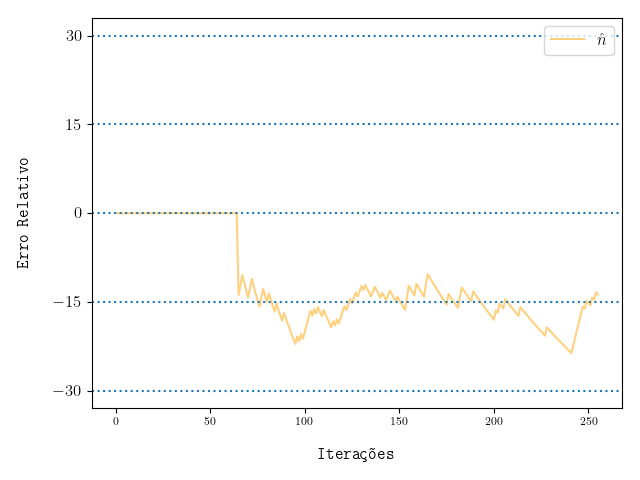
\includegraphics[width=\linewidth, height=4cm]{figuras/adaptive_sampling_erro_first_64.png}
  \end{subfigure}%
  \begin{subfigure}{.5\textwidth}
    \centering
    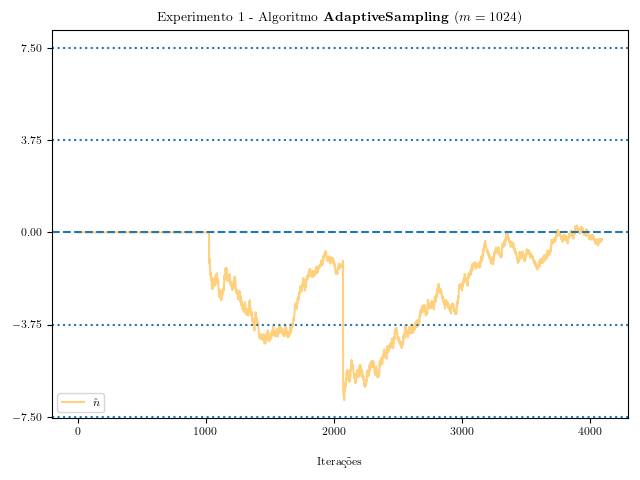
\includegraphics[width=\linewidth, height=4cm]{figuras/adaptive_sampling_erro_first_1024.png}
  \end{subfigure}
  \caption{Erro relativo nas primeiras iterações do experimento do algoritmo~$\AS$. Nas $m$ inserções iniciais,o erro 
  relativo do algoritmo é zero.}
  \label{fig:as:experimento:01:erro:first}
\end{figure}

Para o segundo experimento, repetimos as simulações anteriores dez mil vezes. No final do processo, construímos 
histogramas a partir das frequências das estimativas devolvidas. A Figura~\ref{fig:as:experimento:02:64} tem a 
distribuição das estimativas da estrutura~\texttt{AdaptiveSampling} com $m = 64$ e a 
Figura~\ref{fig:as:experimento:02:1024}, com $m = 1024$. Nos dois casos, quase todos as estimativas ficaram dentro de
dois desvios padrões, e houve uma grande concentração de estimativas entre um desvio padrão. E podemos notar que com um
valor de $m$ maior, a variância do algoritmo das $\asampling$ diminuiu.

\begin{figure}
  \centering
  \begin{subfigure}{.5\textwidth}
    \centering
    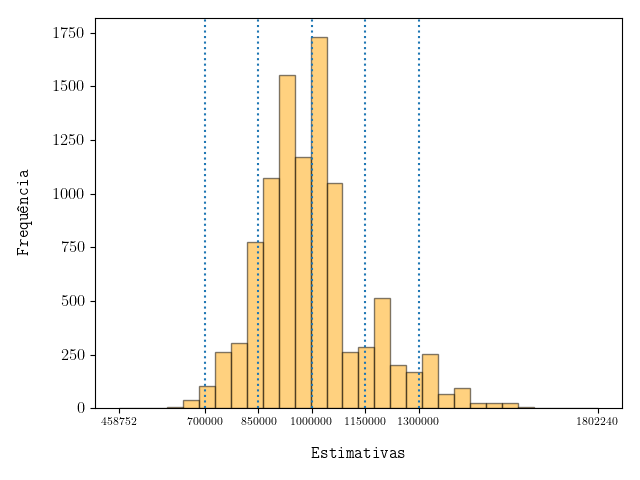
\includegraphics[width=\linewidth, height=4cm]{figuras/adaptive_sampling_variance_64.png}
    \caption{$m = 64$}
    \label{fig:as:experimento:02:64}
  \end{subfigure}%
  \begin{subfigure}{.5\textwidth}
    \centering
    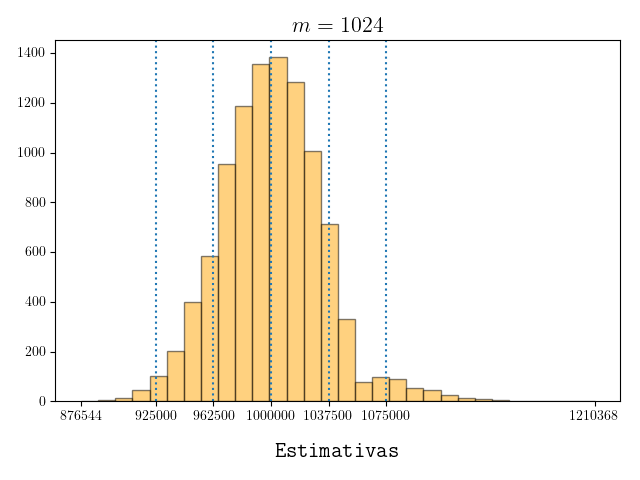
\includegraphics[width=\linewidth, height=4cm]{figuras/adaptive_sampling_variance_1024.png}
    \caption{$m = 1024$}
    \label{fig:as:experimento:02:1024}
  \end{subfigure}
  \caption{Segundo experimento do algoritmo $\AS$. Foram realizadas dez mil simulações e em cada simulação, foram 
    inseridos em estruturas~\texttt{AdaptiveSampling} com $m = 64$ e $m = 1024$, um milhão de inteiros de~64 bits 
    gerados uniformemente. Os resultados foram utilizados para a construção dos histogramas de frequência acima. }
  \label{fig:as:experimento:02}
\end{figure}

Com os experimentos apresentados nessa seção, foi possível termos noção da precisão do algoritmo das~$\asampling$. Este
algoritmo tem pontos interessantes, como se basear em padrões de bits para construir a estimativa e funcionar bem para
fluxos com poucos elementos. Porém, a principal desvantagem dessa solução é o consumo de memória. Se considerarmos uma
aplicação que precise lidar com hashes de 32~bits, então o consumo de memória da estrutura~\texttt{AdaptiveSampling} 
seria de pelos menos $32 \times m$~bits no pior caso, quando a lista $LIST$ passa a ter mais que $m$ elementos. Esse
custo é o mesmo que o do algoritmo~$\pcounting$, quando $L = 32$. Dessa forma, as $\asampling$, que tem um desvio maior
que a $\pcounting$, tem também um consumo de espaço pior. 

Para que esse gasto de memória fosse reduzido sem que se perdesse muita precisão, demorou mais de 20 anos desde a 
criação da $\pcounting$. Veremos na próxima seção como podemos reduzir ainda mais esse consumo.
